\begin{figure}
\centering
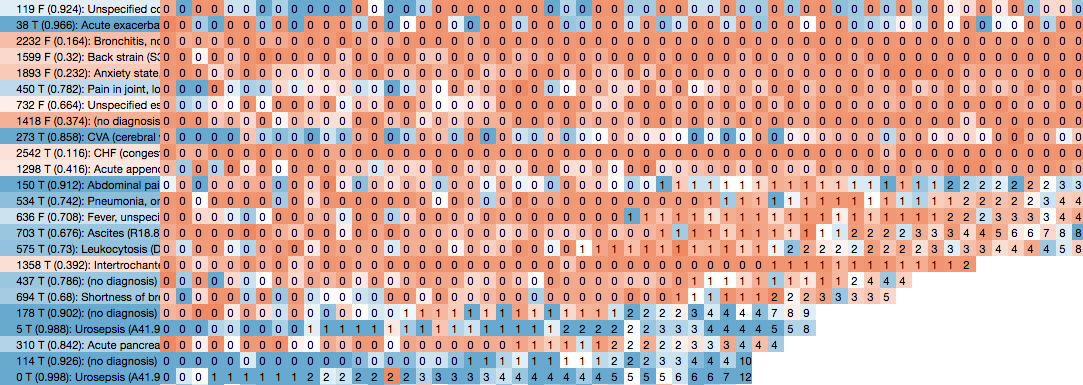
\includegraphics[width=\linewidth]{figs/current/adj_top}
\caption{
Neighborhoods of data points.
Each row represents one neighborhood with its representative (the point with the
highest prediction score) shown on the right.
Each cell represents one data point of the neighborhood.
The background color indicates the prediction score.
The numbers show how many changes in the feature vector are necessary to turn the
point into the representative.
}
\label{figs:current_adj}
\end{figure}